%%%%%%%%%%%%%%%%%%%%%%%%%%%%%%%%%%%%%%%%%%%%%%%%%%%%%%%%%%%%%%%%
% Contents: Math typesetting with LaTeX
% $Id$
%
% Changes by Stefan M. Moser: 2008/10/22
%
% -Section 2: "Single Equations": added comment about preference of
%  equation* over \[
% -Replaced (almost) all examples with \[ by equation*
% -New section 4: "Single Equations that are Too Long: multline"
% -New section 5: "Multiple Equations"
% -Section 6: "Arrays and Matrices": made a full section and added
%  some material
% -Section 9: "Theorems, Lemmas, ...": added a subsection about proofs
%  with new material
%
% Other Changes:
% -in lshort.sty: 
%    *example environment adapted: changed in three places
%     \textwidth by \linewidth. This is necessary for
%     example-environment within a itemize-list.
%    *added \RequirePackage[retainorgcmds]{IEEEtrantools}
%
% THINGS TO DO:
% -adapt typesetting of new sections to rest of lshort, including all
%  the usual commands used so far. In particular, I guess we have to
%  get rid of the \verb-commands everywhere
% -include index-commands
%%%%%%%%%%%%%%%%%%%%%%%%%%%%%%%%%%%%%%%%%%%%%%%%%%%%%%%%%%%%%%%%%
 
\chapter{Results}

\section{Results}
\subsection{Databases:} 
Four databases from SYNTHIA \cite{Ros2016TheSYNTHIA} are used. The selected databases are constructed under different environment conditions: (1) spring, (2) fog, (3) rain and (4) heavy-rain. Moreover, their segmented images, which are provided by the same database, are found to be useful for manually determining the appropriate code of each track. Examples from the four databases are given in Table \ref{Table:Environments_Examples}.	

All implementations were performed by employing a computer with the following facilities: 8 GB RAM and Intel Core i5 processor (3.2 GHz). Only the microprocessor was used in this study to train and test the DRL-RT. The number of frames that have been utilized here are: 270, 284, 268 and 248 frames for the environments of spring, fog, rain and heavy-rain, respectively. The frames are equally divided between the training and testing stages (50\% each), where the odd frames are used in the training stage and the even frames are used in the testing stage.

\begin{figure}[!t]
	\centering
	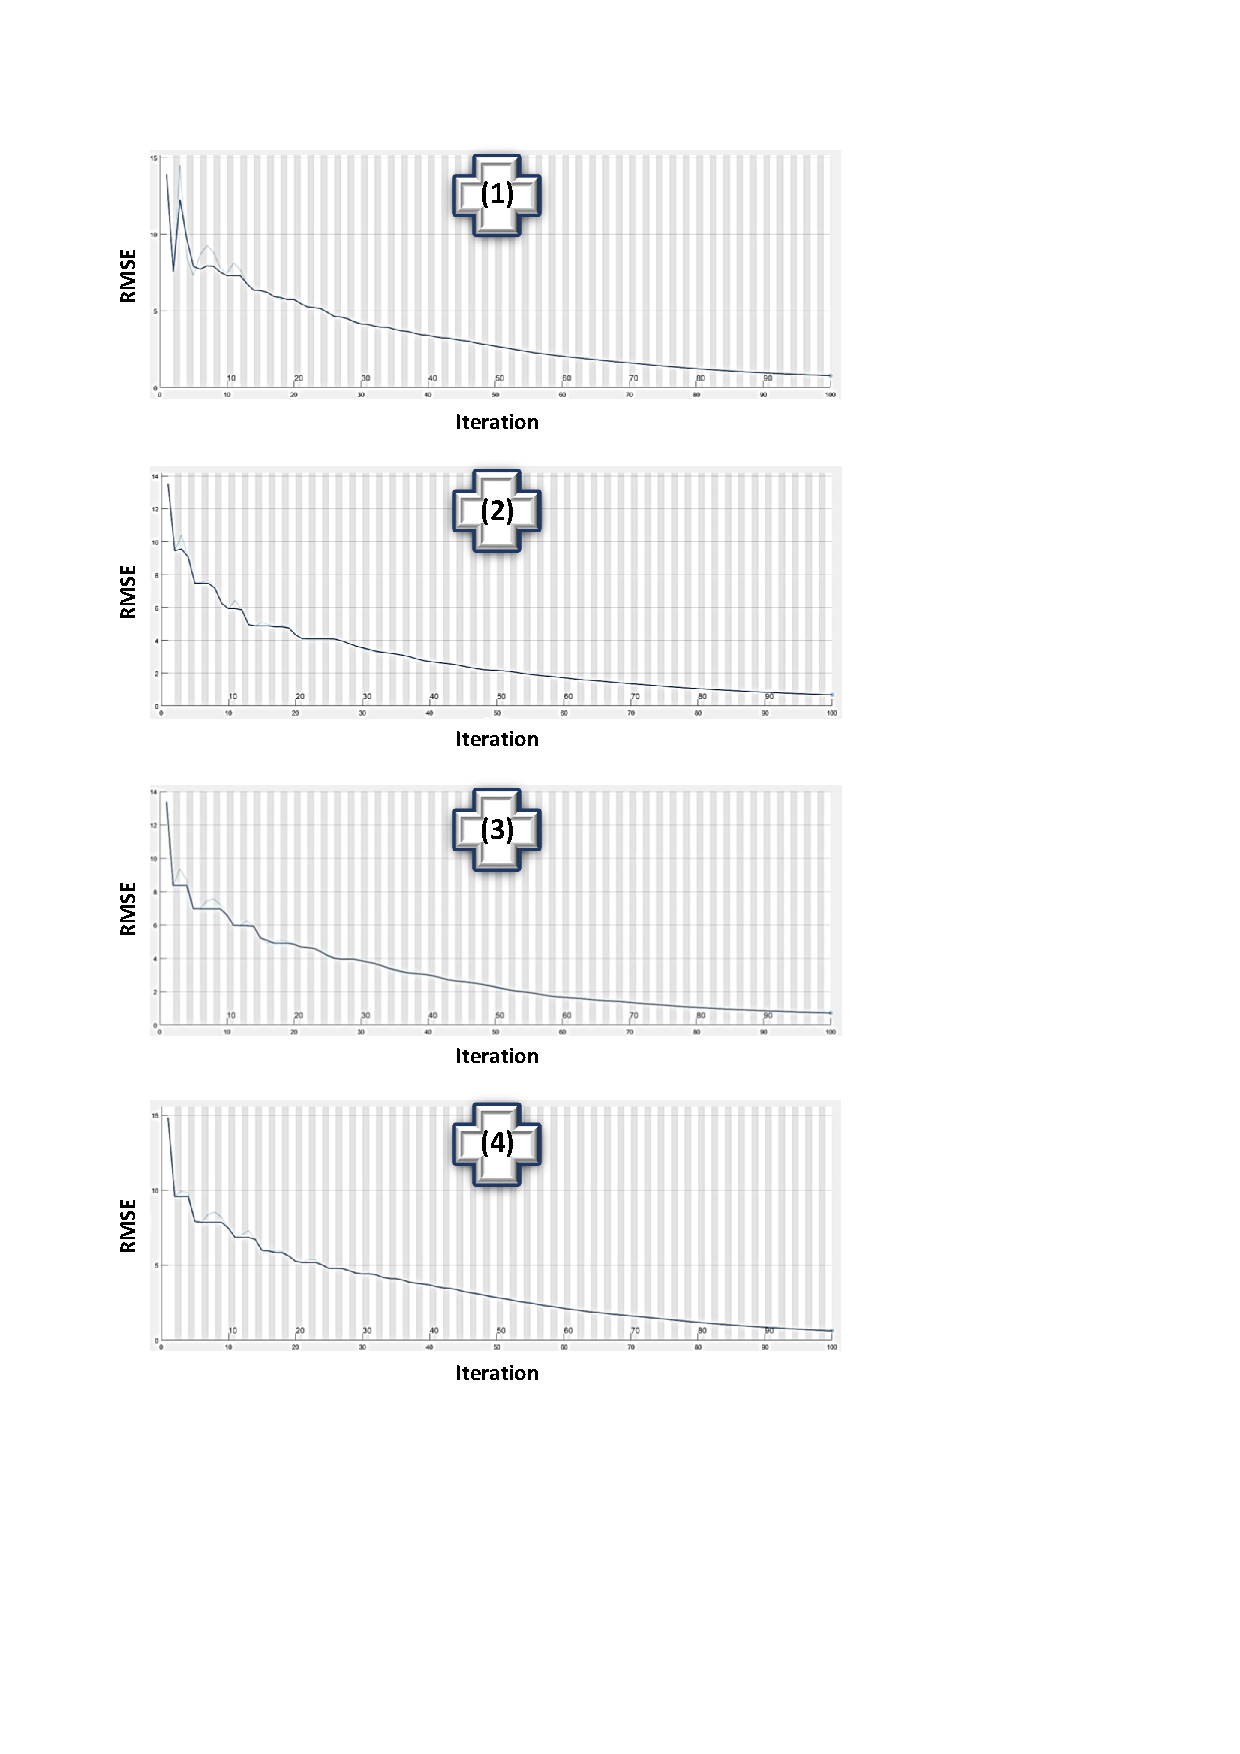
\includegraphics[scale=.67,trim=2cm 6cm 6.5cm 2cm,clip]{training_curves.pdf}
	\caption{The training performance of the DRL-RT for the: (1) spring environment, (2) fog environment, (3) rain environment and (4) heavy-rain environment}
	\label{fig:training_curves}
\end{figure}

\subsection{Training stage:} 
The suggested DRL-RT network has been separately trained for each environment. The following parameters have been assigned for the trainings: Adaptive Moment Estimation (ADAM) optimizer \cite{kingma2014adam}, learning rate equal to 0.0003, gradient decay factor ($\beta_1$) equal to 0.9, squared gradient decay factor ($\beta_2$) equal to 0.99 and mini batch size equal to 128. The training performance of the DRL-RT for the four databases are given in Fig. \ref{fig:training_curves}. This figure demonstrates the relationships between the Root Mean Square Error (RMSE) and the training iterations during the training stages. The RMSE values are usually exploited to demonstrate the differences between desired values and output values.	These differences are usually reduced during the proceeding of training itrations. Clearly, the curves are successfully declined toward goals.

\subsection{Testing stage:} 
The results of the testing stages are interested as it can be observed in Fig. \ref{fig:Main_Results}. To illustrate, the driving accuracy attained its highest value of 93.94\% by using the spring environment database. This is because that the DRL-RT has analysed very clear provided images.  The fog environment database obtained a high driving accuracy of 93.66\%. Here, the overall views are blurred but the road tracking can still be distinguished. The DRL-RT could recognize the road tracking but with slightly lower accuracy than the spring views. The driving accuracy of the rain environment database achieved 89.55\% and this is due to the noise effects of rain drops on image views. Finally, the inferior driving accuracy of 84.68\% was recorded for the heavy-rain environment database as the amount of rain drops (or noise) are increased here.
\begin{figure}[!t]
	\centering
	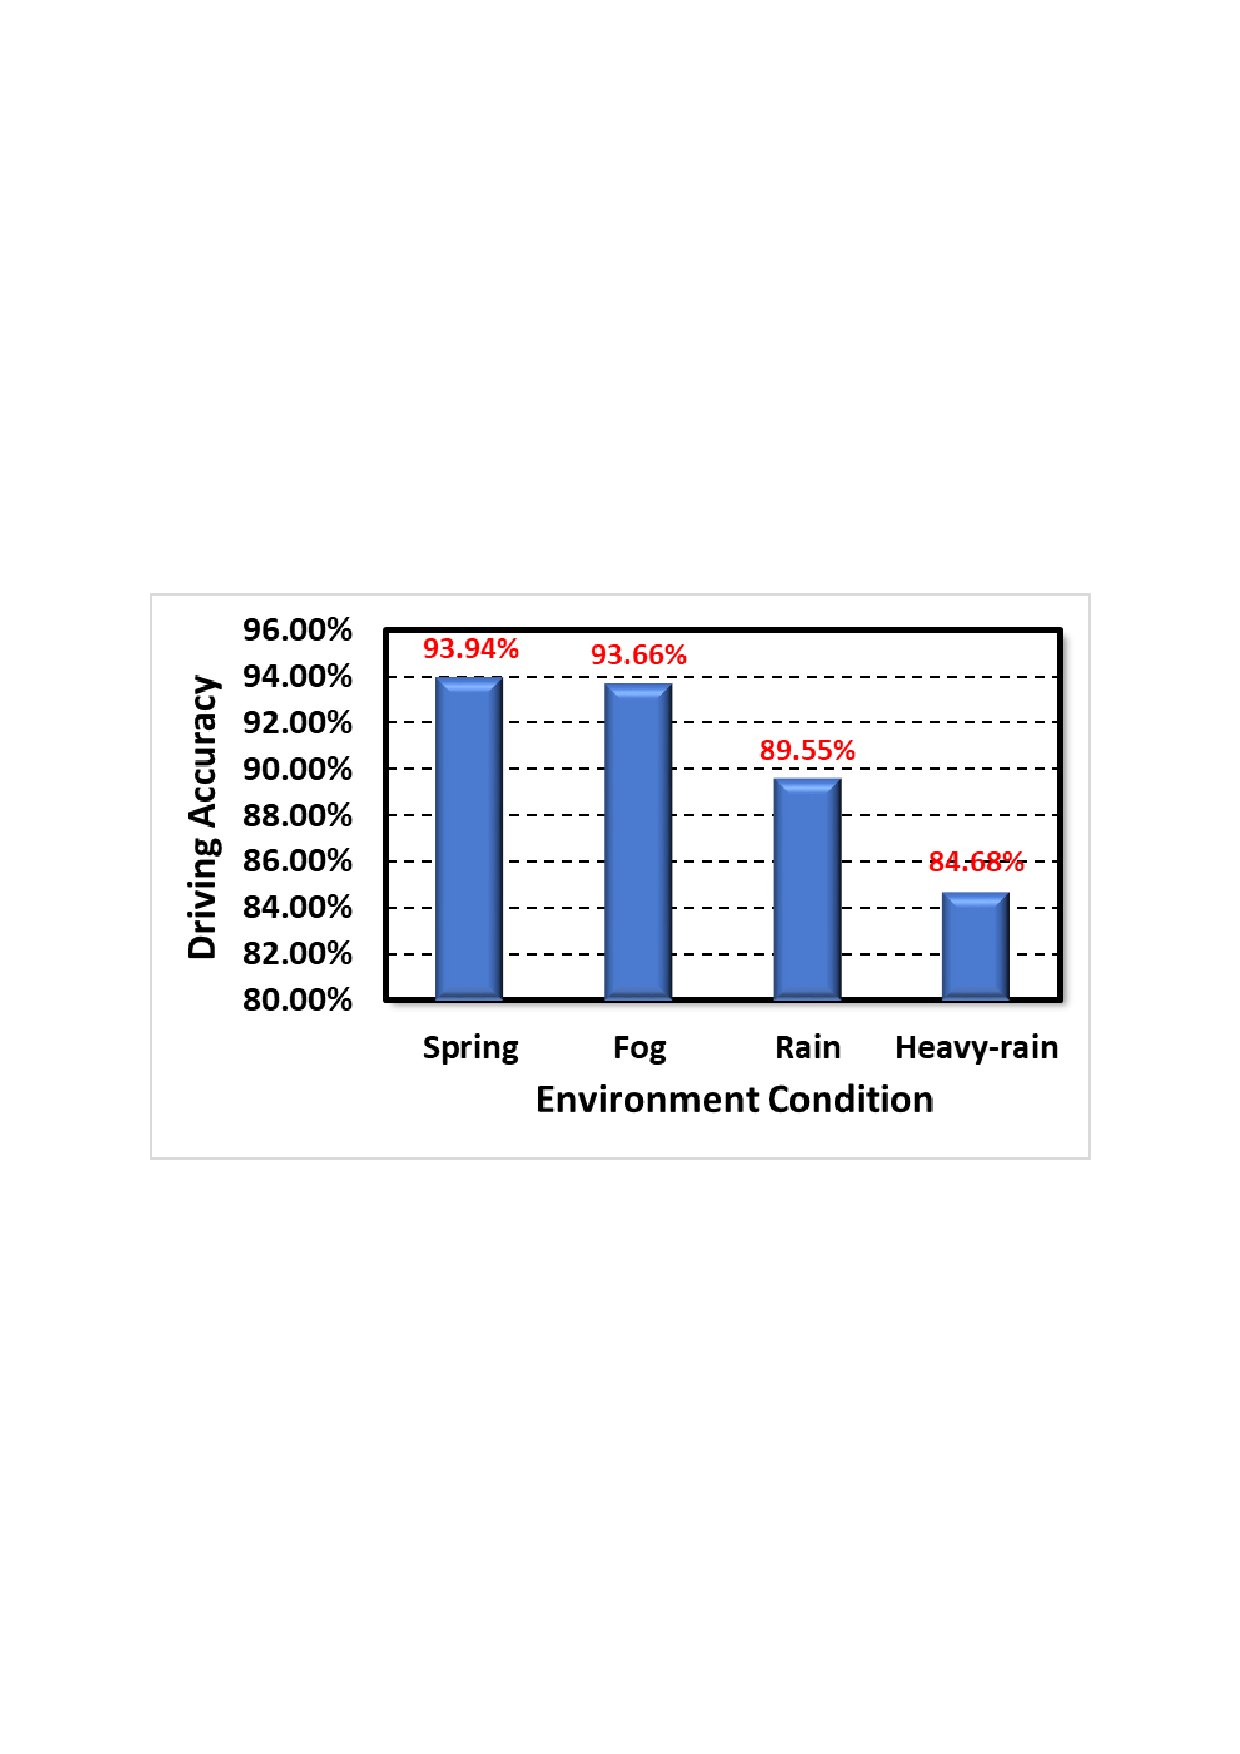
\includegraphics[scale=.58,trim=3cm 10.3cm 2.7cm 10.3cm,clip]{Main_Results.pdf}
	\caption{The performance of the DRL-RT under different employed environments}
	\label{fig:Main_Results}
\end{figure}

\subsection{Comparisons:} 
In the case of comparisons, hard efforts were performed to investigate and simulate various deep learning approaches. Comparisons have been established between our proposed DRL-RT method and other suggested networks. Table \ref{Table:Comparisons} shows the accuracies of different deep learning networks by applying the database of SYNTHIA-SEQS-05-SPRING, some parameters were reasonably changed to allow acceptable comparisons. The reason of selecting this database here is that it has the clear environment, which is suitable to discard undesired effects and provide fair judgement.

\begin{table}[]
	\centering
	\caption{A comparison between our proposed DRL-RT method and other suggested networks}
	\label{Table:Comparisons}
	\begin{tabular}{|C{3cm}|c|c|}
		\hline
		\textbf{Reference} & \textbf{Deep learning method} & \textbf{Accuracy} \\ \hline
		Karaduman and Eren \cite{Karaduman2017Deep} & CNN & 67.42\% \\ \hline
		Bojarski \textit{et al.} \cite{bojarski2016end} & CNN & 74.24\% \\ \hline
		George and Routray \cite{George2016Real} & CNN & 83.33\% \\ \hline
		Yun \textit{et al.} \cite{Yun2017Action,Yun2018Action} & ADNet & 83.33\% \\ \hline
		Mnih \textit{et al.} \cite{mnih2015human} & DQN & 88.64\% \\ \hline
		Proposed method & DRL-RT & 93.94\% \\ \hline
	\end{tabular}
\end{table}

From Table \ref{Table:Comparisons}, it can be seen that the suggested CNN in \cite{Karaduman2017Deep} obtained the inferior tracking accuracy of 67.42\%. This is due to the architecture of this network, where it constructed to classify directions of traffic signs. More specifically, a pooling layer was applied after each convolution layer and no ReLU layers were used. This caused compressing and wasting useful extracted features after each convolution layer. The CNN which is used in \cite{bojarski2016end} attained a low accuracy of 74.24\%. The main drawback of this network is that it considers steering angles to be tracked, where this increases the erroneous of obtaining precise outputs. The CNN in \cite{George2016Real} achieved 83.33\%. This is also due to the architecture of this network, which was designed for classifying eye gaze directions. The ADNet which was approached in \cite{Yun2017Action,Yun2018Action} attained the same accuracy of 83.33\%. 
%	The architecture of this network was mainly consists of convolution layers and fully connected layers, this seems not 
The essential problem here is represented by the considered rewards, which were basically designed %after moving objects and not during the moving. 
for recognizing moved objects as the rewards are updated in the stop action. In addition, the Adnet architecture is not so appropriate for road tracking tasks. The Deep Q-Network (DQN), which is proposed in \cite{mnih2015human} and illustrated in \cite{arulkumaran2017brief} achieved reasonable accuracy of 88.64\%. This can be due to the DQN processes, where it combines between the deep network and the Q-learning. This network can be considered as the nearest method to our approach. Finally, our proposed method has shown superior performance by attaining the accuracy of 93.94\%. This can be due to the overall structure of our road tracking method including the network architecture, tracking policy and designed codes.